%%%%%%%%%%%%%%%%%%%%%%%%%%%%%%%%%%%%%%%%%
% Beamer Presentation
% LaTeX Template
% Version 1.0 (10/11/12)
%
% This template has been downloaded from:
% http://www.LaTeXTemplates.com
%
% License:
% CC BY-NC-SA 3.0 (http://creativecommons.org/licenses/by-nc-sa/3.0/)
%
%%%%%%%%%%%%%%%%%%%%%%%%%%%%%%%%%%%%%%%%%

%----------------------------------------------------------------------------------------
%	PACKAGES AND THEMES
%----------------------------------------------------------------------------------------

\documentclass{beamer}
\usepackage{hyperref}
\usepackage{listings}

\mode<presentation> {

% The Beamer class comes with a number of default slide themes
% which change the colors and layouts of slides. Below this is a list
% of all the themes, uncomment each in turn to see what they look like.

%\usetheme{default}
%\usetheme{AnnArbor}
%\usetheme{Antibes}
%\usetheme{Bergen}
%\usetheme{Berkeley}
%\usetheme{Berlin}
%\usetheme{Boadilla}
%\usetheme{CambridgeUS}
%\usetheme{Copenhagen}
%\usetheme{Darmstadt}
%\usetheme{Dresden}
%\usetheme{Frankfurt}
%\usetheme{Goettingen}
%\usetheme{Hannover}
%\usetheme{Ilmenau}
%\usetheme{JuanLesPins}
%\usetheme{Luebeck}
\usetheme{Madrid}
%\usetheme{Malmoe}
%\usetheme{Marburg}
%\usetheme{Montpellier}
%\usetheme{PaloAlto}
%\usetheme{Pittsburgh}
%\usetheme{Rochester}
%\usetheme{Singapore}
%\usetheme{Szeged}
%\usetheme{Warsaw}

% As well as themes, the Beamer class has a number of color themes
% for any slide theme. Uncomment each of these in turn to see how it
% changes the colors of your current slide theme.

%\usecolortheme{albatross}
%\usecolortheme{beaver}
%\usecolortheme{beetle}
%\usecolortheme{crane}
%\usecolortheme{dolphin}
%\usecolortheme{dove}
%\usecolortheme{fly}
%\usecolortheme{lily}
%\usecolortheme{orchid}
%\usecolortheme{rose}
%\usecolortheme{seagull}
%\usecolortheme{seahorse}
%\usecolortheme{whale}
%\usecolortheme{wolverine}

%\setbeamertemplate{footline} % To remove the footer line in all slides uncomment this line
%\setbeamertemplate{footline}[page number] % To replace the footer line in all slides with a simple slide count uncomment this line

%\setbeamertemplate{navigation symbols}{} % To remove the navigation symbols from the bottom of all slides uncomment this line
}

\usepackage{graphicx} % Allows including images
\usepackage{booktabs} % Allows the use of \toprule, \midrule and \bottomrule in tables

%----------------------------------------------------------------------------------------
%	TITLE PAGE
%----------------------------------------------------------------------------------------

\title[Group Meeting Talk]{GEM5 Simulator in Full System Mode} % The short title appears at the bottom of every slide, the full title is only on the title page

\author{Yizi Gu} % Your name
\institute[Department of EE,THU] % Your institution as it will appear on the bottom of every slide, may be shorthand to save space
{
Tsinghua University\\ % Your institution for the title page
\medskip
\textit{yizigu@gmail.com} % Your email address
}
\date{\today} % Date, can be changed to a custom date

\begin{document}

\begin{frame}
\titlepage % Print the title page as the first slide
\end{frame}

\begin{frame}
\frametitle{Overview} % Table of contents slide, comment this block out to remove it
\tableofcontents % Throughout your presentation, if you choose to use \section{} and \subsection{} commands, these will automatically be printed on this slide as an overview of your presentation
\end{frame}

%----------------------------------------------------------------------------------------
%	PRESENTATION SLIDES
%----------------------------------------------------------------------------------------

%------------------------------------------------
\section{Study Background} % Sections can be created in order to organize your presentation into discrete blocks, all sections and subsections are automatically printed in the table of contents as an overview of the talk
\subsection{GEM5 introduction}
\begin{frame}
\frametitle{A modular platform for computer architecture research}
GEM5 is a cycle accurate simulator. It is the combination of two separate
simulator: GEMS and M5. It follows the object oriented design pattern, which
makes the extension of modules relatively easy. There are mainly two running
modes:
\begin{itemize}
    \item SE(System call Emulation): System calls are passed to the host
	machine. 
	\begin{itemize}
	    \item Good for testing/profiling micro-architecture design
	    \item Not enough for assessing the system level performance.
	\end{itemize}
    \item FS(Full System): Simulating a bare metal machine with CPU, memory
	hierarchy, I/O, devices. 
	\begin{itemize}
	    \item More realistic and more interesting than SE mode
	    \item Need appropriate kernel and file system image.
	\end{itemize}
\end{itemize}
\end{frame}
\begin{frame}
\frametitle{Compilation and Module Wrapping}

\begin{itemize}
    \item SCons:  GEM5 is compiled under the control of SCons, a promising substitution for Make.
    \item Swig: A automatic wrapper for connecting C++ with python.  A typical
	auto-generated wrapper function is shown in figure ~\ref{fig:swig}.
	The parameters could be set by python scripts which avoids re-compiling the whole source code.
	\begin{figure}[H]
	    \begin{center}
		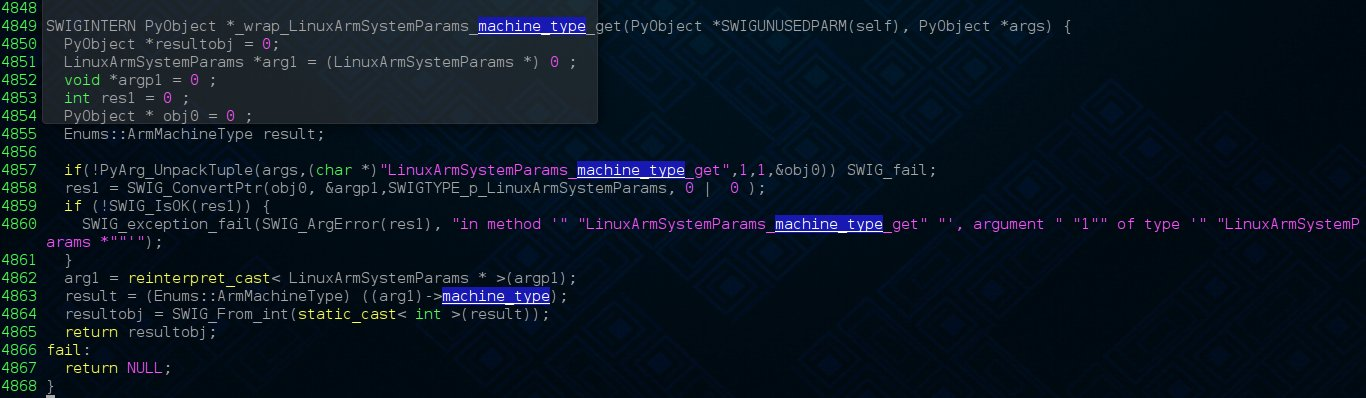
\includegraphics[scale=0.3]{back6.jpg}
	    \end{center}
	    \caption{Swig Wrapper function}
	    \label{fig:swig}
	\end{figure}
\end{itemize}
\end{frame}
\subsection{Application in current research}
%------------------------------------------------
\begin{frame}
\frametitle{Support for Non-Volatile Sensors Architecture Study}
Basic Idea:
\begin{itemize}
    \item Add new device(sensor) in the GEM5 source tree
    \item Write kernel module(driver) to support the new device
    \item Run system benchmark: The benchmark could be generated by using the
	experimental data such as the typical power supply of energy harvesting nodes.
    \item Calculate the metrics and evaluate the architectural design.
\end{itemize}
\end{frame}
\section{Current Progress}
\subsection{OS Basics}


\begin{frame}
\frametitle{The typical boot process of a Linux machine}

\begin{block}{Stage 0}
On start up, the BIOS program fixed in FLASH or motherboard is first executed
and choose the candidate boot device(Hard Disk, Floppy Disk, USB stick etc.)
\end{block}
\begin{block}{Stage 1}
Execute first stage bootloader. If boot from hard disk, the 1st stage
bootloader resides in the first 446 Bytes of the 512-Byte large MBR(Master
Boot Record). The remaining 64 Bytes record four pieces of partition
information. The bootloader makes sure there is one and only one active
partition from which the machine will boot by inspecting these records.
\end{block}
\end{frame}
\begin{frame}
    \frametitle{Cont'd}
\begin{figure}[H]
    \begin{center}
	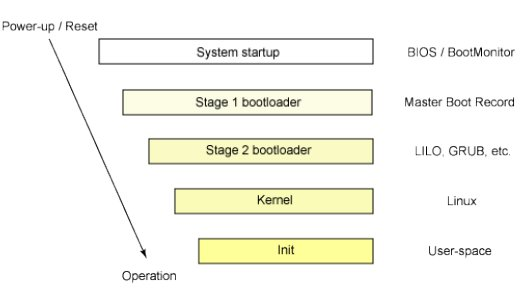
\includegraphics[scale=0.8]{back9.jpg}
    \end{center}
    \caption{Simplified Boot Process}
\end{figure}
\end{frame}

\begin{frame}
    \frametitle{Cont'd}
\begin{block}{Stage 2}
The second stage bootloader is loaded and executed. 1st and 2nd stage
bootloaders are generally called LILO(Linux Loader)/GRUB(GRand Unified
Bootloader). Initial RAM Disk(initrd) will be loaded into the memory and work
as a temperate file system for further booting the complete system.
\end{block}
\begin{block}{Stage 3}
The bootloader then starts the compressed kernel image(zImage/bzImage). And it
decompresses itself by calling several functions in head.S, misc.c. At the end
of the progress, the basic software environment such as stack and page table
are set. Then the start\_kernel() function in init/main.c is called. 
\end{block}
\end{frame}

\subsection{How to make it work}
\begin{frame}
    \begin{itemize}
	\item Download the kernel and disk image from \href{http://www.m5sim.org/Download}{official website}
	\item Currently the kernel vmlinux.arm.smp.fb.2.6.38.8 runs together with disk image linux-arm-ael.img smoothly.
    \end{itemize}
    \begin{figure}[H]
	\begin{center}
	    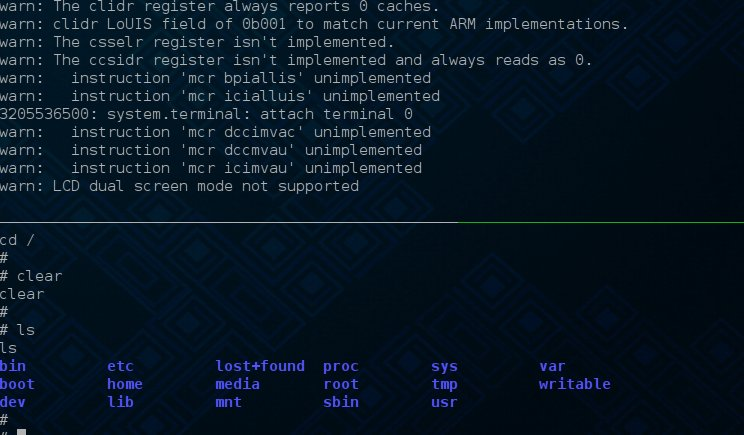
\includegraphics[scale=0.5]{back10.jpg}
	\end{center}
	\caption{FS runtime demonstration}
    \end{figure}
\end{frame}
\subsection{How to add files/programs to the disk image}
\begin{frame}
    \frametitle{How to manipulate the disk image}
    Problem: The disk image is only a bare file system. How to add
    files/programs to the system efficiently? \par Possible Solutions:
    \begin{enumerate}
	\item Connecting the network: May be rather slow.
	\item Boot the system using virtual machine(QEMU/VirtualBox).
	\item Mount the file system locally using mount command.
    \end{enumerate}
    Solution 2 is a good approach but I haven't found the proper kernel and
    disk image which fit GEM5 and QEMU at the same time. So I mount the file
    system directly by the shell command:\par
\qquad	sudo mount -o loop,offset=32256 linux-arm-ael.img /mnt\par
    After mounting the image, we could copy the programs into the file
    tree:\par   
    \qquad sudo cp a.out /mnt/home/\par
\end{frame}

\begin{frame}
    \frametitle{Cont'd}
    We could cross-compile the program on the host machine and then move the
    binaries into the file system for simulation:	
    \begin{figure}[H]
	\begin{center}
	    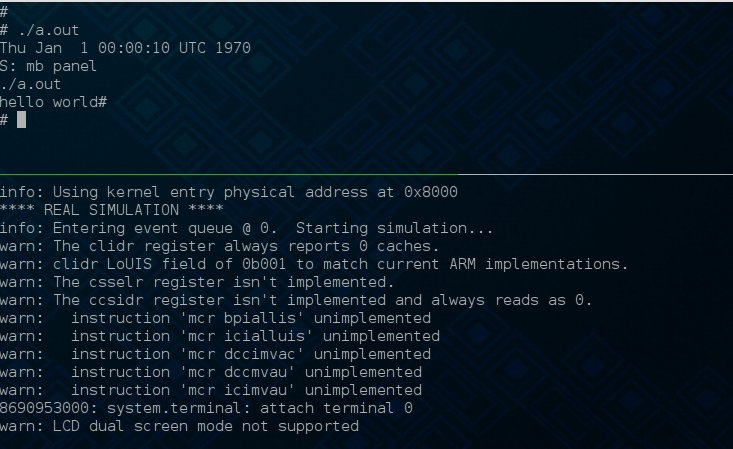
\includegraphics[scale=0.5]{back11.jpg}
	\end{center}
	\caption{FS node running imported program}
    \end{figure}
\end{frame}

\begin{frame}
    \frametitle{Kernel Module}
    I first download the kernel source file whose version is in accordance with
    the current pre-compiled kernel version(2.6.38.8). Then cross-compiling
    the module using the kernel header files downloaded. Then move the .ko
    file into the file system and insert the module. I got a problem with the
    magic version that remains to be solved:
    \begin{figure}[H]
	\begin{center}
	    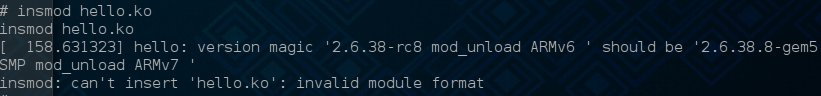
\includegraphics[scale=0.5]{back12.jpg}
	\end{center}
    \end{figure}
\end{frame}

\begin{frame}
    \frametitle{This week's work}
    \begin{itemize}
	\item Study the GEM5 FS mode further and learn how to get the
	    simulation profiles.
	\item Read papers relevant to the research
    \end{itemize}
\end{frame}

\begin{frame}
\Huge{\centerline{Thank you}}
\end{frame}


\end{document} 
